\documentclass[11pt, oneside]{article}   	% use "amsart" instead of "article" for AMSLaTeX format
\usepackage{geometry}                		% See geometry.pdf to learn the layout options. There are lots.
\geometry{letterpaper}                   		% ... or a4paper or a5paper or ... 
%\geometry{landscape}                		% Activate for rotated page geometry
%\usepackage[parfill]{parskip}    		% Activate to begin paragraphs with an empty line rather than an indent
\usepackage{graphicx}				% Use pdf, png, jpg, or eps§ with pdflatex; use eps in DVI mode
								% TeX will automatically convert eps --> pdf in pdflatex		
\usepackage{amssymb}

%SetFonts

%SetFonts

\graphicspath{ {./images/} } 			

\title{Population Pyramids}
\author{M: 941519}
%\date{}							% Activate to display a given date or no date

\begin{document}
\maketitle


\tableofcontents
\pagebreak
\section{Cos'è una "population pyramid"}
Una "population pyramid" è una illustrazione grafica che ci permette di visualizzare la distribuzione di una popolazione (che può essere un paese in particolare, una regione del mondo, o un continente), dividendoli in bracket di anni ed in spezzandoli in segmenti in base alla proporzione tra maschi e femmine.\\

La population pyramid è formata quindi da una serie di barre ad istogramma, la popolazione è rappresentata dalla grandezza dell'asse orizzontale, ed i bracket di anni sono rappresentati dall'asse $y$.


\begin{center}
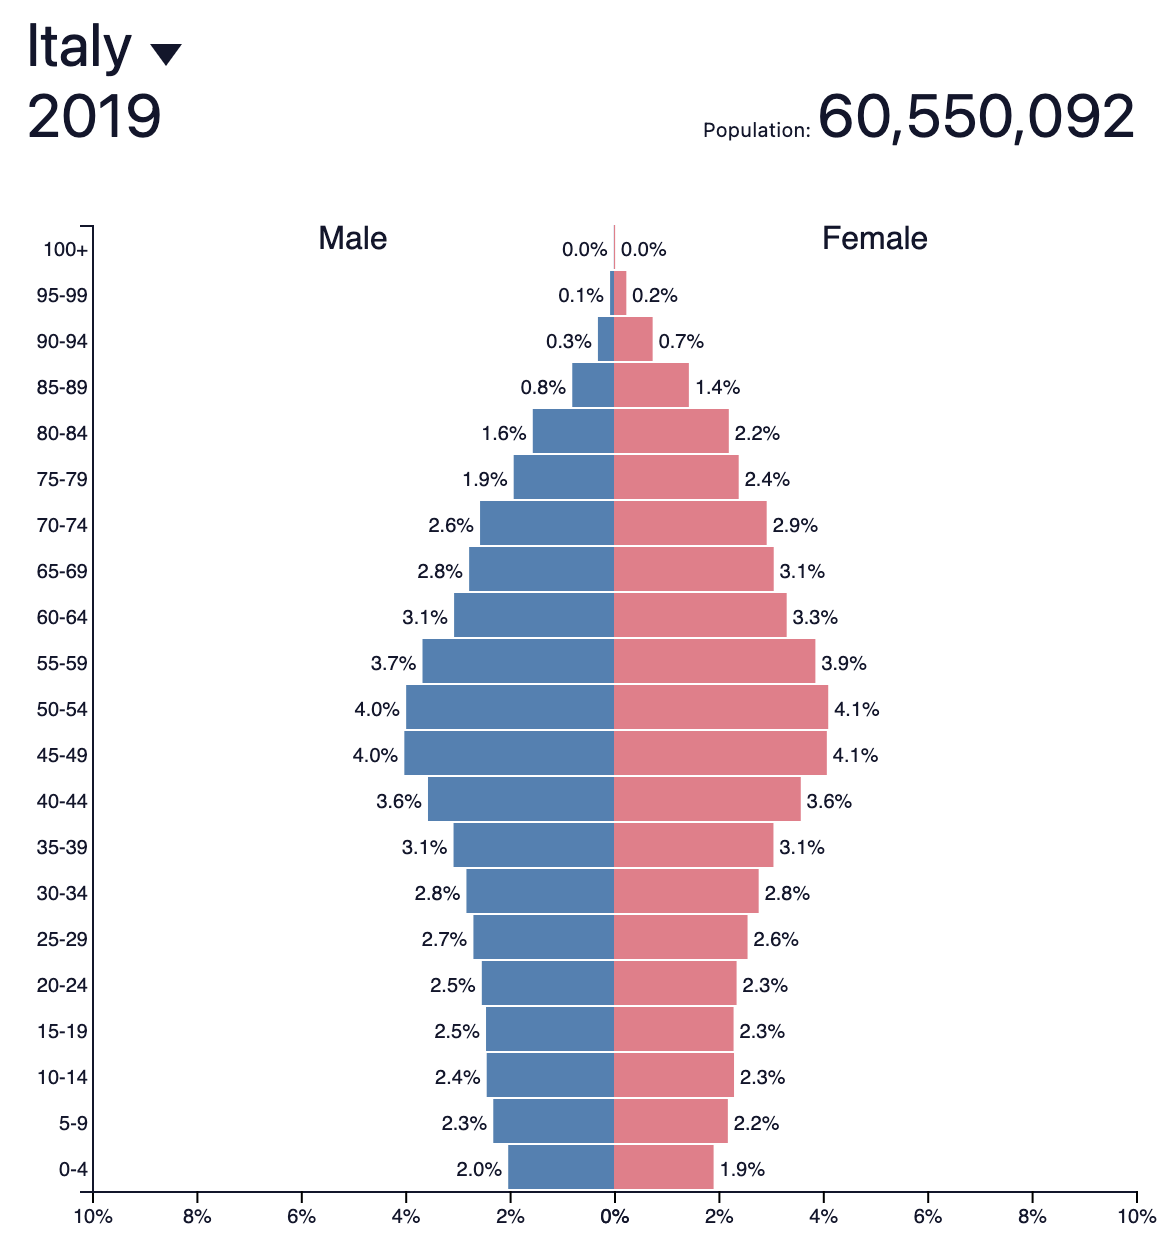
\includegraphics[scale=0.6]{pop}
\end{center}

\subsection{Perché è chiamata una "piramide"?}
L'origine del nome deriva dalla forma che questo grafico ha assunto per la maggior parte della vita dell'uomo, ovvero quella della piramide:

\begin{center}
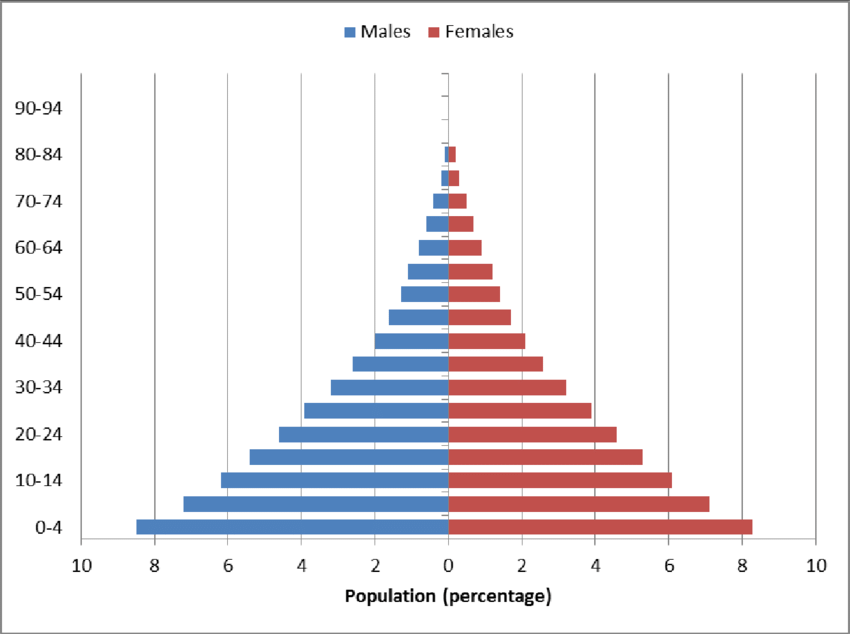
\includegraphics[scale=0.5]{pyramid.png}
\end{center}

Formata da una forma chiaramente piramidale, senza buoni contraccettivi e con una popolazione poco educata, la popolazione cresce man mano che ci spostiamo verso il basso del grafico, le famiglie sono composte da molti bambini, che in parte non raggiungono neanche i vent'anni, e la popolazione diminuisce progressivamente per la mancanza di buona medicina e prevenzione. Quella comunque, è la "population pyramid" dell'Africa Subsahariana.


\section{I dati necessari per costruire una "population pyramid"}
Per costruire una population pyramid abbiamo bisogno prima di tutto della popolazione totale in uno specifico anno, nel nostro esempio abbiamo preso l'Italia nell'anno 2019, e la popolazione totale è di $60.550.092$. \\
Il secondo dato fondamentale che ci serve è la proporzione, rispetto alla popolazione totale, della popolazione per ogni "age bracket". Questo dato va a rispondere alla domanda: \emph{"quante persone, maschio e femmina, vi erano, in percentuale, rispetto alla popolazione totale ?"}. Questo dato ci permette di dimensionare le varie barre del nostro grafico\\
L'ultimo dato fondamentale è la proporzione tra maschi e femmine, rispetto ad ogni "age bracket", che ci permette dimensionare, in proporzione, i maschi e le femmine.

\section{Esempio di costruzione utilizzando python}
Utilizziamo un dataset fornito da \emph{https://www.populationpyramid.net/}:
\begin{center}
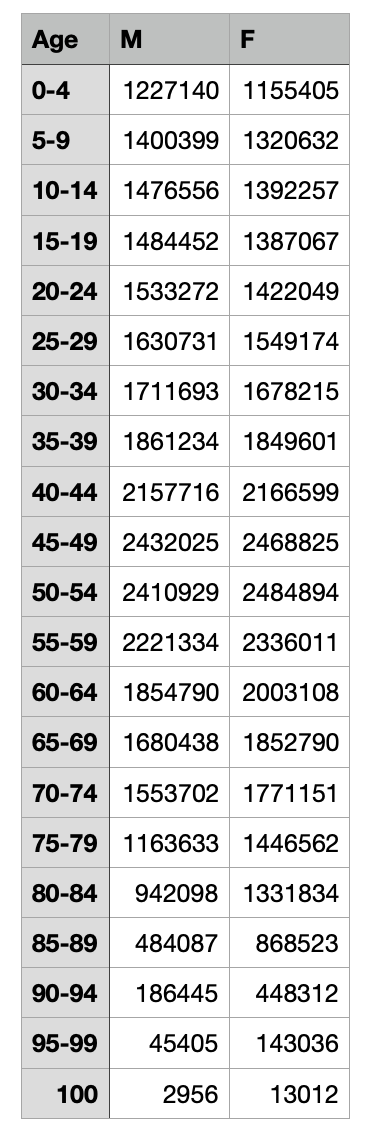
\includegraphics[scale=0.6]{popitaly}
\end{center}
Andiamo ad importare il dataset all'interno del notebook:
\begin{center}
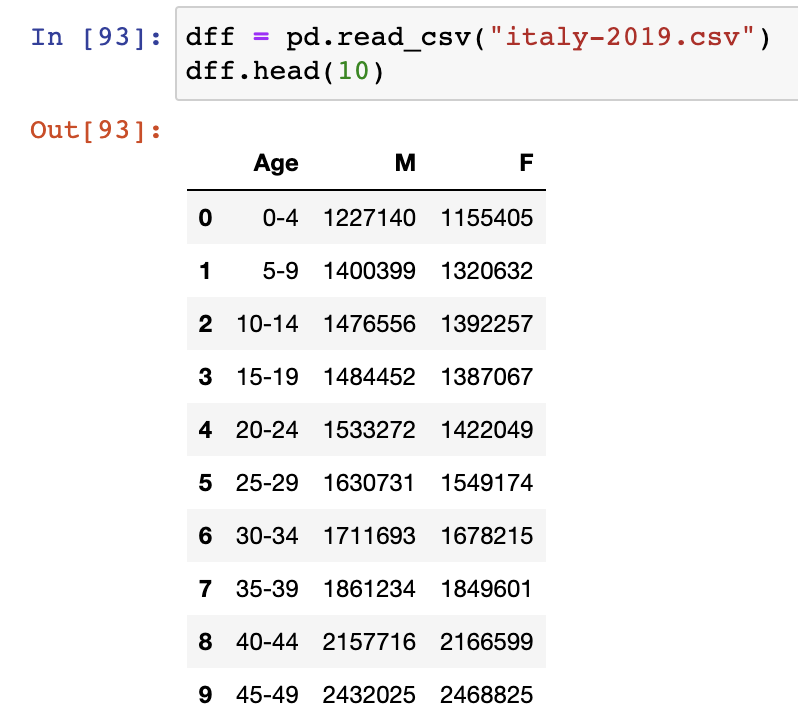
\includegraphics[scale=0.6]{popitaly2}
\end{center}
Costruiamo due liste, una per i maschi ed una per le femmine, raccogliendo i valori in base all'age bracket:
\begin{center}
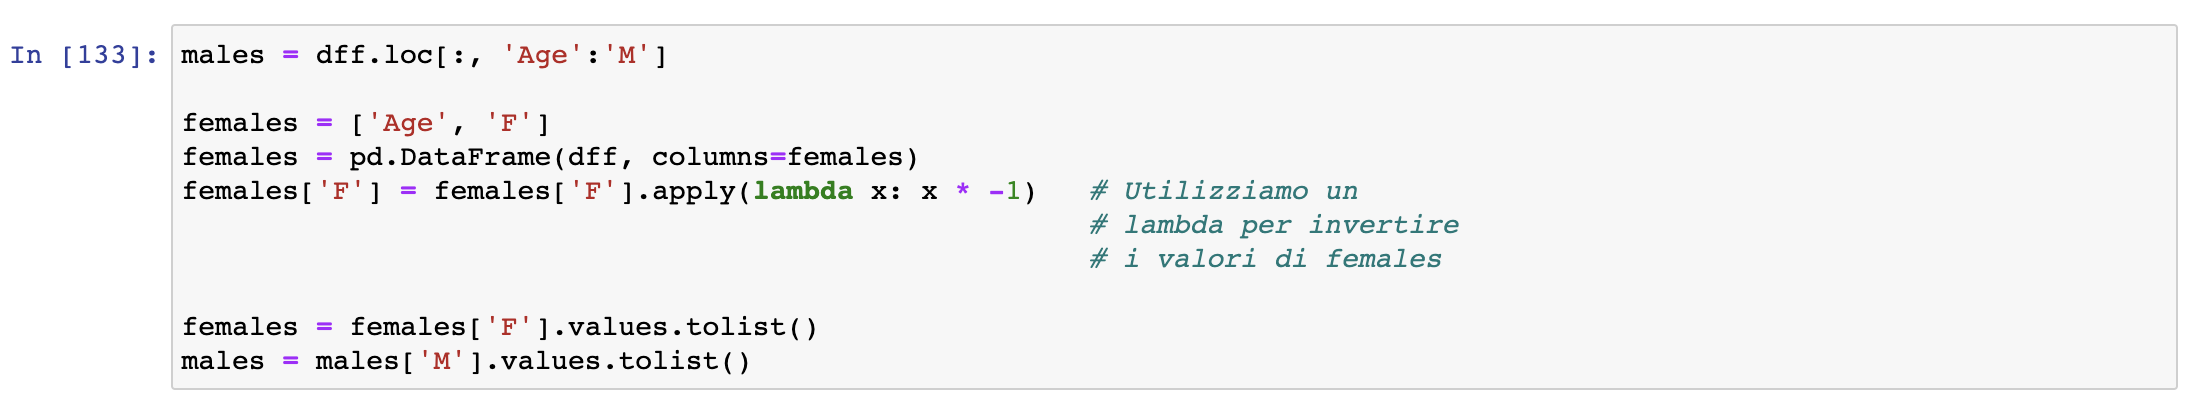
\includegraphics[scale=0.4]{popitaly3}
\end{center}
Creiamo un dataframe con headers: "Age", "Males", "Females", e utilizziamo le liste precedentemente create come input. utilizziamo quindi la libreria seaborn (basata su matplotlib) per creare la nostra population pyramid:
\begin{center}
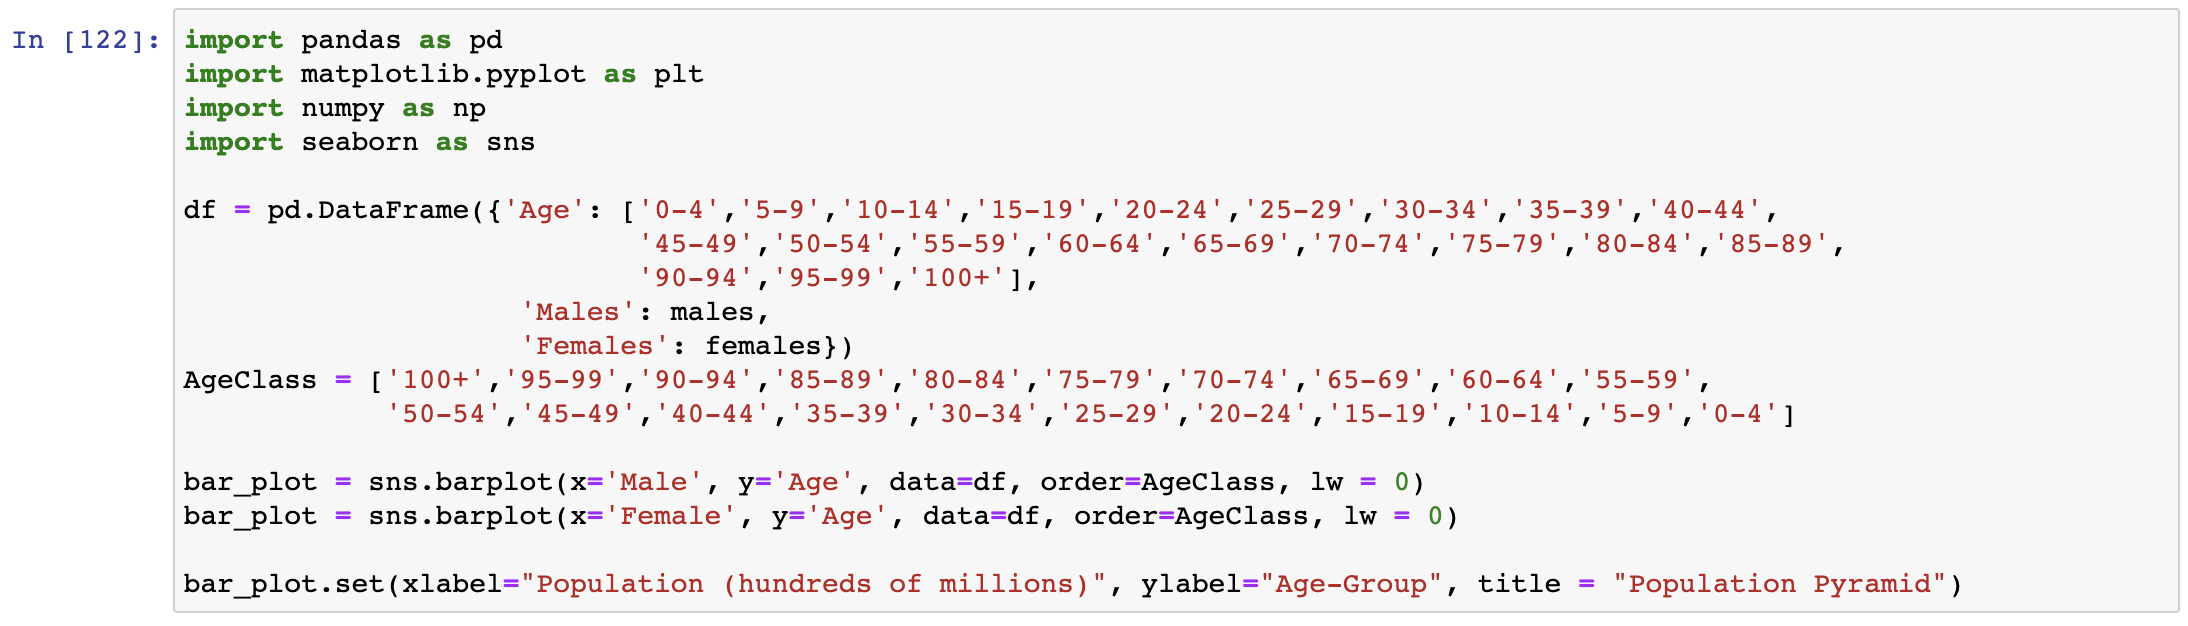
\includegraphics[scale=0.4]{popitaly4}
\end{center}
Il risultato finale è il seguente:
\begin{center}
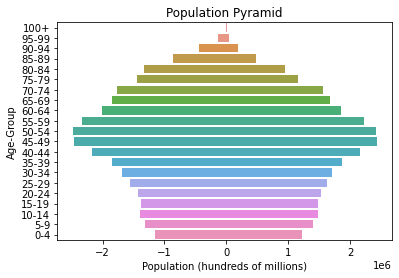
\includegraphics[scale=1]{popitaly5}
\end{center}
%\subsection{}

\section{I tipi di population pyramid}
\begin{itemize}


\section{Cosa ci dice una "population pyramid"}
\subsection{Un'appendice sull'età}
\emph{Qual'è il miglior indicatore per prevedere il comportamento di una "persona media" ed il suo contributo alla società?}\\
Ci sono molte risposte a questa domanda, il background culturale, la professione, le condizioni sociali, le norme e gli usi e costumi di un paese. L'europeo medio ad esempio risparmia di più rispetto ad un americano medio, il finanziere che gudagna 100.000\$ l'anno investe di più (anche solo perché ha più disposable income) di un meccanico che raggiunge a malapena il fine mese, e così via.\\
C'è tuttavia un dato che ci permette di prevedere, in maniera pressoché accurata, il contributo di una persona al proprio paese, l'età.

\subsubsection{Perché l'età è un indicatore così importante}
Utilizziamo la nostra "population pyramid", e consideriamo la bracket di popolazione con età superiore a 65 anni circa. Questa categoria è rappresentata solitamente dai pensionati, che hanno terminato la propria carriera lavorativa, spendono poco, investono in maniera prudente e non contribuiscono più alle casse dello stato. \\

Il secondo gruppo che ci interessa è la bracket di popolazione con età compresa tra i 30 e i 65 anni. Questo bracket di popolazione rappresenta il "motore" di un paese, rappresenta il lavoratore medio che percepisce uno stipendio, spende, risparmia, e contribuisce alle casse dello stato. Durante questi anni la persona media raggiunge il massimo potenziale economico, facendo carriera, comprando case, macchine, e mettendo su famiglia. E' questo quindi il motivo per cui possiamo considerare questo bracket di popolazione come la risorsa più importante di un paese, più importante anche delle risorse naturali, e della posizione geografica.\\

Il terzo gruppo che ci interessa è la bracket di popolazione con età compresa tra i 15 ed i 30 anni. Questo bracket di popolazione è principalmente composta da persone che stanno per terminare la propria carriera formativa, e che stanno per entrare nel mondo del lavoro.
Durante questi anni la persona media non guadagna molto, vive solitamente con i genitori, e ha bisogno di prestiti per finanziare rette universitarie, o per comprare la prima casa.\\

L'ultimo gruppo che ci interessa è la bracket di popolazione con età inferiore ai 15 anni. Questo bracket di popolazione è la "più inutile" per un paese, formata da studenti e bambini che non contribuiscono ad una economicamente ad una società, ed invece costano molto alle famiglie sotto forma di mantenimento, pannolini etc.

\section{Indicatori complementari}
\begin{itemize}
\item Dependancy ratio
\end{itemize}

\section{Estensione delle population pyramids}
\begin{itemize}
\item Population pyramid colorate maschio e femmina\\
L'abbiamo vista in precedenza, ed è la più semplice delle varianti, sono population pyramids in cui le barre sono colorate a seconda del sesso della popolazione.
\item Population pyramid con surplus
Sono un'estensione della precedente, in cui oltre al colorare il sesso delle barre, coloriamo in maniera differente il surplus delle barre rispetto all'altro sesso, in questo modo possiamo visualizzare in maniera semplice la quantità di maschi, o femmine, in più in un paese.
\begin{center}
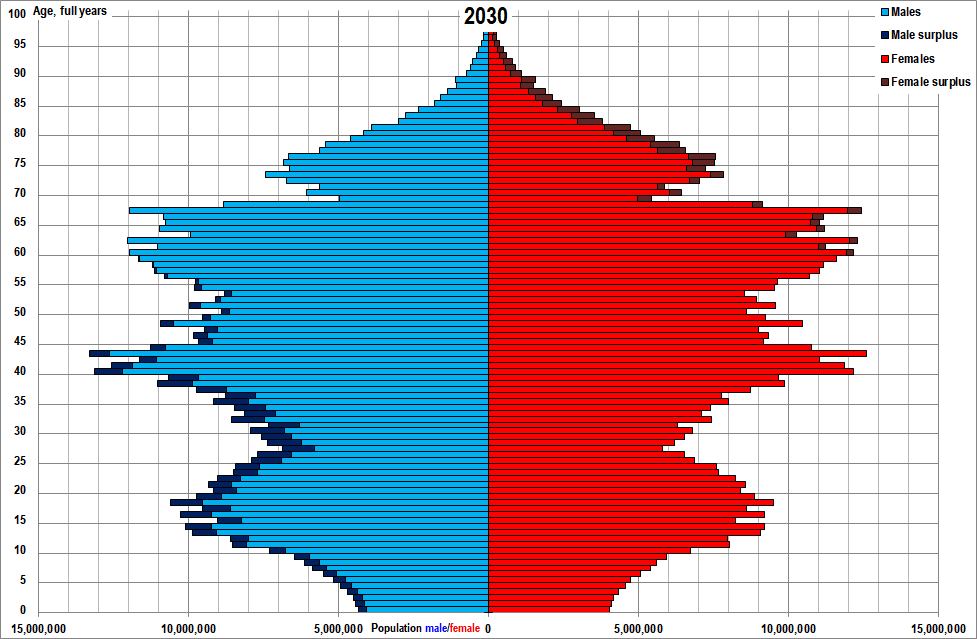
\includegraphics[scale=0.6]{china}
\end{center}
\item Animazioni con population pyramids\\
Andiamo a costruire un'animazione con il dataset che abbiamo.
Siccome il nostro dataset va dal 2000 al 2020, estendiamo il programmino creato in precedenza aggiungendo un ciclo range, e salviamo con nome ogni grafico prodotto, dal 2000 al 2020.

\begin{center}
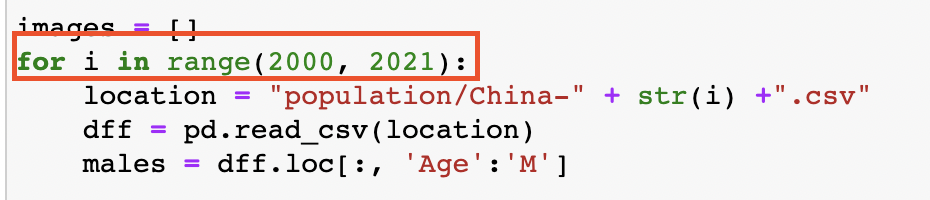
\includegraphics[scale=0.5]{china1}


\includegraphics[scale=0.55]{china2}

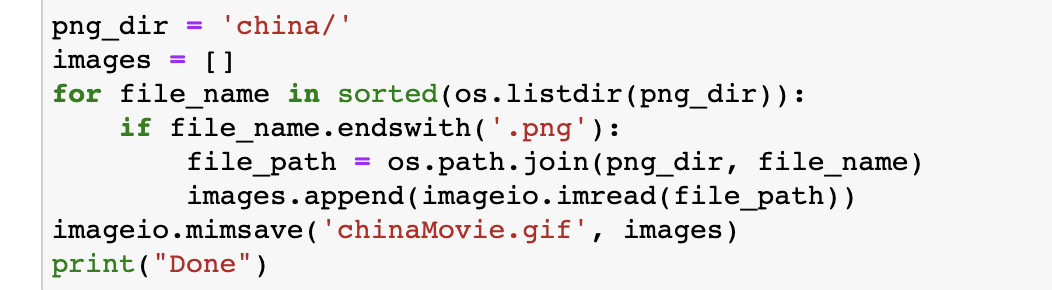
\includegraphics[scale=0.5]{china3}
\end{center}
Con le immagini generate utilizziamo un piccolo script basato su \emph{imageio} per generare una .gif.\\
Questo tipo di animazione ci permette di vedere in maniera dinamica lungo gli anni l'andamento della popolazione, in particolare possiamo vedere come la popolazione -nei paesi in via di sviluppo-, si sposta tendenzialmente verso l'alto allontanandosi sempre più da una piramide, ed avvicinandosi ad una campana; mentre nei paesi il cui l'indice di sviluppo è basso il grafico rimane una piramide, indicatore di come lo sviluppo non stia tenendo passo.

\item Predizioni sul futuro con population pyramids\\
Un qualcosa che ci stanno pregando di fare le animazioni precedenit è quello di estenderle, per darci una visione del futuro. In base all'andamento demogrifco di un paese è quindi possibile estendere il grafico lungo gli anni.

\end{itemize}













\end{document}  